\documentclass[a4paper]{article}

% Support for Norwegian letters
\usepackage[latin1]{inputenc}
\usepackage[T1]{fontenc}
\usepackage{amsmath,amsfonts,amssymb,amsthm,booktabs,array,mathtools}
% consider package mhchem for typesetting chemical formulas
\usepackage{graphicx} % Why isn't this here by default?

% Proper space and font for integral differential term
\newcommand{\dd}{\; \mathrm{d}} 
% Shorcut for ODEs with proper font
\newcommand{\diff}[2]{\frac{\mathrm{d} #1}{\mathrm{d} #2}}
% Shortcut for PDEs with proper font (shortcut: PDB)
\newcommand{\pdiff}[2]{\frac{\partial #1}{\partial #2}}
\newcommand{\pdiffn}[3]{\frac{\partial^{#3} #1}{\partial #2^{#3}}}

% Absolute value and norm commands.
% Read the mathtools.pdf to fix these!
\providecommand{\abs}[1]{\lvert#1\rvert} 
\providecommand{\norm}[1]{\lVert#1\rVert}

% Set the depth of section numbering
\setcounter{secnumdepth}{0}

\begin{document} 

We found signals of polyadenylation events in the GENCODE cell lines by
trimming and remapping those reads that were originally unmappable and ended in
a stretch of As or beginning with a stretch of Ts. We subsequently merged the
polyadenylation sites into clusters in a similar way to Tian et. al
\cite{tian_large-scale_2005}. In total, for all cell lines and compartments, we
obtained 29860 polyadenylation sites with support of 2 or more reads or falling
at annotated polyadenylation sites.  17125 of these were found in 3UTR regions.
To compare our findings with annotated polyadenylation sites, we first merged
and clustered 43187 sites from the polyAdb with 35791 sites from GENCODE to
obtain a total of 50696 annotated polyA sites. 16657 of our polyA sites fall at
annotated ones (81\% or 13517 of these are in 3UTRs), leaving a total of 13203
putative novel polyadenylation sites in the genome. Table XX shows an overview
over the number of poly(A) sites in different genomic regions.

Since the RNA-seq protocol for the Gingeras data is not optimized for 3' ends,
we expected to find most poly(A) sites for transcripts with high RPKM. To
measure this, we calculated the ratio of discovered to annotated poly(A) sites
in the 3UTRs of transcripts with non-overlapping 3UTRs. Figure \ref{fig:RPKM}
shows the relationship between RPKM and poly(A) discovery ratio for annotated
3UTRs. As can be seen, there is a positive relationship between RPKM and
poly(A) discovery (r = 0.52, p < $10^{-10}$), however there is considerable
variation even for high RPKM transcripts (we considered an RPKM of minimum 0.5
to count as expressed). The average number of poly(A) sites found per 3UTR was
1.7, and the average ratio of poly(A) sites to annotated was 0.9, probably
reflecting both that the method is not exhaustive, and that not all annotated
poly(A) sites are used by transcripts at a given time.

\begin{figure}[h]
	\centering
		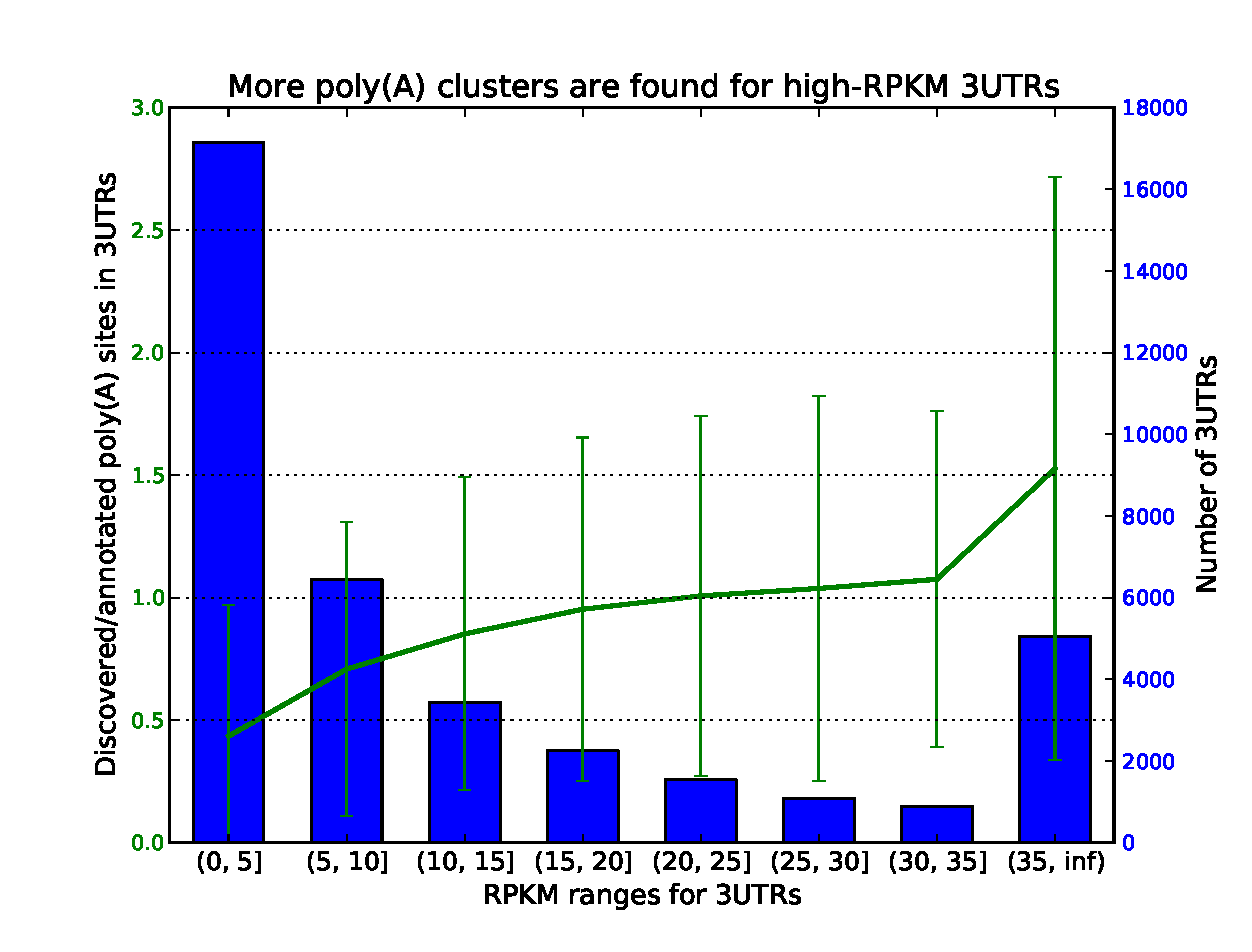
\includegraphics[scale=0.5]{../Figures/More_polyA_clusters_for_high_RPKM_3UTRS.eps}
	\caption{RPKM-poly(A) discovery link}
	\label{fig:RPKM}
\end{figure}

\subsection{Polyadenylation in the nucleus and in the cytoplasm}

We wanted to compare poly(A) sites in the nucleus and cytoplasm. While poly(A)
sites in the nucleus are expected to derive from from the 3' ends of stable,
multi-copy mRNA, the poly(A) sites from the nucleus are expected to stem from
mRNA diffusing toward the cytoplasm, mRNA undergoing processing, and possibly
some RNA undergoing degradation
\cite{shcherbik_polyadenylation_2010,slomovic_addition_2010}.

We merged the poly(A) sites from 5 cell lines in the nucleus and cytoplasm
separately for the poly(A)+ and poly(A)- fractions and
compared the distribution of the polyadenylation sites in the genome (Figure
YYXYXY). The division of RNA between poly(A)+ and poly(A)- happens at an
average of 30(A) residues.

\subsubsection{Poly(A)- vs poly(A)+ in the nucleus and cytoplasm}
In Figure X A), it can be seen that there are found proportionally a larger
fraction of poly(A)- reads in the nucleus than in the cytoplasm.
The polyadenylation marks in the cytoplasmic poly(A)- fraction can
come from mRNA that is being degraded (as the poly(A) tail is gradually
decreased in length before degradation), which will be discussed below..

As can be seen, the nuclear regions capture polyadenylation signals both in the
poly(A)+ and poly(A)- fractions in the intronic regions. Intronic
polyadenylation has been identified for many genes \cite{}TIAN, which could
explain that markers of polyadenylation is found in the poly(A)+ fraction.
However, it was unexpected to find polyadenylation markers in the poly(A)-
fraction. Their presence in this fractions means that they originate from RNA
that had a poly(A) tail of 30nt or less. ?? Keep?This could be the evidence of a
different type of adenylated RNA in the nucleus, such adenylation as a marker
for degradation \cite{}.??

It can be seen that for the poly(A)+ fraction the whole-cell samples are most
similar to the cytoplasmic ones. However, while the over-all numbers are lower for
the nucleus compared to the cytoplasm and whole cell, the relative distribution of
poly(A) reads in the different genomic regions is the same. This could indicate that
previous studies of polyadenylation that have used whole cell extracts and
poly(A)+ fractions have given conclusions that are representative for both the
cytoplasm and the nucleus.

In the poly(A)- fraction it can be seen that it is the nucleus that has more
marks of polyadenylation than the cytoplasm. In other words, it seems that
there is more adenylation with short poly(A) tails in the nucleus compared to
the cytoplasm. For some of the adenylation sites in the 3UTR this difference
could be explained by polyadenylation caught-in-action, however it does not
explain the increase in the other genomic reagions.

To investigate whether the markers of polyadenylation we observe are in the
sense or anti-sense to anntated genomic features, we looked at only those
genomic regions that have features in one sense uniquely, and that do not
overlap with any other genomic features. Table XXX shows this. Discuss this.

Given the recent reports of degradation-related adenylation in humans, we
looked for signatures of degradation. Marks of adenlyated assisted degradation
are expected to be less reproducable and less location-specific than 3' mRNA
polyadenylation, although in \cite{} the adenylation sites were frequently
found at identical or close-by locations both in the nucleus and in the
cytoplasm. Any degrdation-related adenylation site would not be likely to
contain the PAS-signal downstream, which XXX\% of annotated polyadenylation
sites in 3UTRs do (Table 1). Thus we searched for adenylation sites that were
not at annotated sites and that did not contain one of the PAS downstream.
Since degradation-related (A)-tails are shorter than the ones found at the 3'
end of mRNAs, these tails are expected to be represented with reads from the 3'
pair-end read, thus being originally found with a poly(T) header. Further, as
well as genuine poly(A) signals, they are expected to map to the sense strand.
Table XXX contains an overview of all polyadenylation sites without PAS. As can
be seen $\dots$. Is the increase in poly(A)- adenylation in the nucleus to the
cytoplasm due to non-PAS adenylation for all regions? Would be great.

1 TODO make the big table you mention about in the first part
2 TODO make the unique sense-antisense libraries and make sure they don't
overlap each other. Return similar values as for polyadenylation, but now
include K562 nucleoplasm and chromatin as well (actually you can include them
in the above too).

DISCUSSION

1) It's possible to use conventional RNA-seq to study polyadenylation, you just
need a lot of reads.

2) Evidence for geniune poly(A) reads lie in the strandedness of the reads and
the A/T origin of the reads. Long tails may have A-endings, but probably few,
while short A-tails are expected to have only Ts.

3) Difference in nucleus/cytoplasm for poly(A)+/-. 

\bibliographystyle{plain}
\bibliography{/users/rg/jskancke/phdproject/bibtex/jorgsk}
%\bibliography{/home/jorgsk/work/bibtex/jorgsk}

\end{document}


